\documentclass[tikz,border=5]{standalone}
\usetikzlibrary{matrix,arrows,positioning,shadows}
\tikzset{
    feature/.style={draw, inner sep=1.5mm, font=\small\sffamily, fill=white, drop shadow},
    opt/.style={fill=white}}

\begin{document}

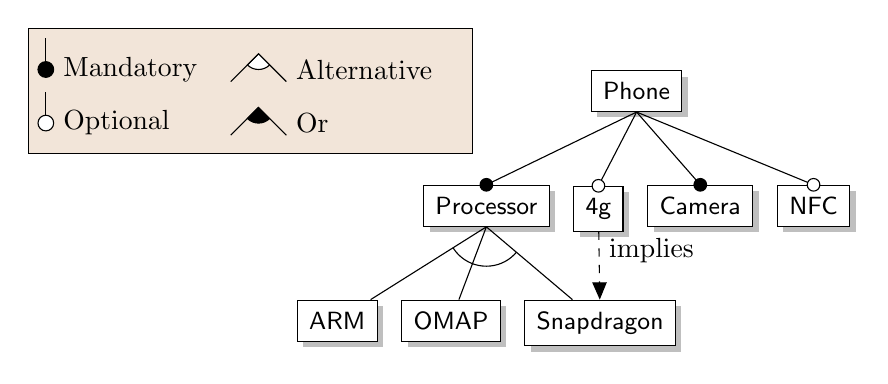
\begin{tikzpicture}[
  node distance=.8cm,
  legendtext/.style={text width=2cm}]
  \node[feature] (phone) {Phone};

  \matrix (sub)[matrix of nodes,
                below=of phone,
                column sep=3mm, row sep=0mm, nodes=feature]{
  Processor & %sub-1-1
  4g & %sub-1-2
  Camera & %sub-1-3
  NFC \\ %sub-1-4
  };

  \matrix (group)[matrix of nodes, 
                  below=of sub-1-1,
                  column sep=3mm, row sep=0mm, nodes=feature]{
  ARM & %group-1-1
  OMAP & %group-1-2
  Snapdragon \\ %group-1-3
  };

  \draw (phone.south) -- (sub-1-1.north);
  \draw (phone.south) -- (sub-1-2.north);
  \draw (phone.south) -- (sub-1-3.north);
  \draw (phone.south) -- (sub-1-4.north);

  \draw (sub-1-1.south) -- (group-1-1);
  \draw (sub-1-1.south) -- (group-1-2);
  \draw (sub-1-1.south) -- (group-1-3);

  %cross-tree constraint
  \draw[-triangle 45,dashed] (sub-1-2) -- (group-1-3)
    node[pos=.6,anchor=south west] {implies};

  %optional / mandatory
  \draw[opt] (sub-1-2.north) circle (.8mm); 
  \draw[opt] (sub-1-4.north) circle (.8mm); 
  \fill[draw] (sub-1-1.north) circle (.8mm); 
  \fill[draw] (sub-1-3.north) circle (.8mm); 

  %Group arc
  \begin{scope}
    \path[clip] (sub-1-1.south) -- (group-1-1.center) -- (group-1-3.center) -- cycle;
    \draw (sub-1-1.south) circle (.5cm);
  \end{scope}

\matrix [draw=black,fill=brown!20,left=1.5cm of phone] {
  \node[fill=black,draw,circle,inner sep=2pt,outer sep=0pt] (m) at (0,0){}; \draw (m) -- +(0,0.4); & \node[legendtext]{Mandatory}; & 
   \filldraw[fill=white,draw=black] (0,0.2) -- ++(225:0.2) arc[start angle=225,end angle=315,radius=0.2]; 
 \draw (0,0.2) ++(225:0.5) -- (0,0.2) -- ++(315:0.5);& \node[legendtext]{Alternative}; \\
  \node[fill=white,draw=black,circle,inner sep=2pt,outer sep=0pt] (o) at (0,0){}; \draw (m) -- +(0,0.4); & \node[legendtext]{Optional}; & 
  \draw (0,0.2) ++(225:0.5) -- (0,0.2) -- ++(315:0.5);
  \filldraw[black] (0,0.2) -- ++(225:0.2) arc[start angle=225,end angle=315,radius=0.2]; & \node[legendtext]{Or}; 
\\
};
\end{tikzpicture}
\end{document}